\documentclass{beamer}
\usetheme{Boadilla}
% \usepackage{beamerthemesplit} // Activate for custom appearance


\setbeamertemplate{navigation symbols}{}
\setbeamertemplate{footline}{}

\usepackage{gensymb}
\usepackage[absolute,overlay]{textpos}
\usepackage{braket}
\usepackage{bm}

\title{Tunable Testbed for Detection and Attribution}
\subtitle{IDAG Workshop 2018}
\author{Nathan Lenssen}
\institute{Columbia University, Department of Earth and Environmental Sciences \\
		Lamont-Doherty Earth Observatory}
\date{March 14, 2018}

\titlegraphic{\vspace*{1.5cm} 
\includegraphics[height=1cm]{Images/ldeoLogo.png}\hspace*{4.75cm}~%
   
\includegraphics[height=1cm]{Images/nsfLogo.jpg}
}

\newcommand{\Prob}{\ensuremath{\mathbb{P}}}
\newcommand{\E}{\ensuremath{\mathbb{E}}}
\newcommand{\V}{\ensuremath{\text{Var}}}
\newcommand{\C}{\ensuremath{\text{Cov}}}
\newcommand{\insitu}{\emph{in situ }}
\newcommand{\iid}{\ensuremath{\stackrel{\text{iid}}{\sim}}}

\setbeamerfont{framesource}{size=\tiny}

\newcommand{\source}[1]{\begin{textblock*}{4cm}(0.1 cm,8.9cm)
    \begin{beamercolorbox}[ht=0.5cm,left]{framesource}
        \usebeamerfont{framesource}\usebeamercolor[fg]{framesource} Source: {#1}
    \end{beamercolorbox}
\end{textblock*}}

% shortcut for bold
\def\*#1{\bm{#1}}
\def\C{\textbf{\text{C}}}
\def\W{\textbf{\text{W}}}

\begin{document}

\frame{\titlepage}


%%%%%%%%%%%%%%%%%%%%%%%%
% (I) Introduce formulation used in presentation
%%%%%%%%%%%%%%%%%%%%%%%%

%%%
% (A) EIV formulation
%%%

% OLS
\begin{frame}
\frametitle{Statistical Formulation of Detection and Attribution}
\framesubtitle{Ordinary Least Squares (OLS)}

\structure{Observed Quantities:}
\begin{itemize}
\item[$\*y$:] The \alert{observed} climate response of interest 
\item[$\*X^*$] The \alert{model-simulated} forcing responses $\*X^* = (\*x^*_1, \dots, \*x^*_m , \dots, \*x^*_M)$
\end{itemize}

\begin{block}{}
\vspace*{-5pt}\setlength\belowdisplayshortskip{0pt}
\begin{equation*}
\*y = \*X^* \*\beta + \* u
\end{equation*}
\end{block}

\structure{Statistical Parameter of Interest:}
\begin{itemize}
\item[$\*\beta$] Estimation provides detection, inference (CIs)  gives us attribution
\end{itemize}

\structure{Climate Variability:}
\begin{itemize}
\item[$\*u$] The error due to climate variability where $\*u \sim \mathcal{N}(0, \C)$
\item[$\C$] Estimated through model control runs
\end{itemize}
\end{frame}

% EIV model 1: Introduction
\begin{frame}
\frametitle{Statistical Formulation of Detection and Attribution}
\framesubtitle{Error-in-Variable (EIV)}
\structure{Observed Quantities:}
\begin{itemize}
\item[$\*y$] The climate response of interest 
\item[$\*X$] The \alert{noisy} responses to forcings $\*X = (\*x_1, \dots, \*x_m , \dots, \*x_M)$
\end{itemize}

\begin{block}{}
\vspace*{-\baselineskip}\setlength\belowdisplayshortskip{0pt}
\begin{align*}
\*y &= \*X^* \*\beta + \*u_y \nonumber \\
\*X &= \*X^* + \*U \:
\end{align*}
\end{block}

\structure{Latent Quantities:}
\begin{itemize}
\item[$\*y^*$] The `true' climate response where $\*y^* = \*X^* \*\beta$
\item[$\*X^*$] The `true' responses to forcings $\*X^* = (\*x_1^*, \dots, \*x_M^*)$
\end{itemize}

\structure{Climate Variability:}
\begin{itemize}
\item[$\*u_y$] As OLS formulation with $\*u_y \sim \mathcal N(0, \C)$
\item[$\*U$] The error on the forcing responses due to climate variability
\setlength\abovedisplayskip{0pt}
\setlength\belowdisplayskip{0pt}
\[
\*U = (\*u_1, \dots, \*u_M) \stackrel{\text{iid}}{\sim} \mathcal{N}(0,\C)
\]

\end{itemize}

\end{frame}

% EIV model 2: Multimodel ensembles
\begin{frame}
\frametitle{Statistical Formulation of Detection and Attribution}
\framesubtitle{Error-in-Variable (EIV): Multimember Ensembles}

For a given forcing $m$, we run ensemble of size $L_m$
\[
\*x_m = ( \*x_m^{(1)}, \dots \*x_m^{(\ell)}, \dots, \*x_m^{(L_m)}) \, , \qquad  \*x_m^{(\ell)} \iid \mathcal{N}(\*x^*_m, \C)
\]

The \structure{ensemble mean} of the $m^{\text{th}}$ forced response is 
\begin{align*}
\overline{\*x_m} &= \frac{1}{L_m} \sum_{\ell=1}^{L_m} \*x_m^{(\ell)} \, , \qquad  \overline{\*x_m} \sim \mathcal{N}\left(\*x^*_m, L_m^{-1}\,\C\right)
\end{align*}

Rewriting in the error-in-variable formulation
\[
\overline{\*x_m} = \*x^*_m +L_m^{-1/2} \*u_m
\]
Or for all forcing responses with $\*L = \text{diag}(L_1, \dots, L_M)$
\begin{exampleblock}{}
\vspace*{-5pt}\setlength\belowdisplayshortskip{0pt}
\[
\overline{\*X} = \*X^* +\*L^{-1/2} \*U
\]
\end{exampleblock}
\end{frame}


% EIV Model 3: Incoporation of multimodel ensembles
\begin{frame}
\frametitle{Statistical Formulation of Detection and Attribution}
\framesubtitle{Error-in-Variable (EIV): Multimember Ensembles}

\begin{exampleblock}{}
\vspace*{-5pt}\setlength\belowdisplayshortskip{0pt}
\[
\overline{\*X} = \*X^* +\*L^{-1/2} \*U
\]
\end{exampleblock}

Plugging into our full error in variable formulation:

\begin{block}{}
\vspace*{-\baselineskip}\setlength\belowdisplayshortskip{0pt}
\begin{alignat*}{3}
\*y &= \*X^* \*\beta + \*u_y \nonumber  \qquad  &\*u_y &\sim \mathcal N(0,\C) \\
\overline{\*X} &= \*X^* + \*L^{-1/2} \*U \qquad    &\*u_m &\iid \mathcal N(0,\C)  \:
\end{alignat*}
\end{block}

\begin{itemize}
\item[$\overline{\*X}$] The ensemble means $\overline{\*X} = (\overline{\*x_1}, \dots, \overline{\*x_M})$ 
\item[$\*L$] The ensemble sizes $\*L = (L_1, \dots, L_M)$
\item[$\*U$] The forcing variability matrix $\*U = (\*u_1, \dots, \*u_M)$
\end{itemize}
\end{frame}

%%%
% (A) obs formulation
%%%

% true, realize, observed responses
\begin{frame}
\frametitle{Statistical Formulation of Detection and Attribution}
\framesubtitle{Observed Response Variability}

The \alert{incomplete} expression for the climate response $\*y$ is
\begin{alertblock}{}
\vspace*{-5pt}\setlength\belowdisplayshortskip{0pt}
\begin{equation*}
\*y = \*X^* \*\beta + \* u_y  \, , \qquad \*u_y \sim \mathcal{N} (0,\C) 
\end{equation*}	
\end{alertblock}

We propose three different $\*y$ states to fully incorporate all of the sources of variability.

\begin{itemize}
\item[$\*y^*$] The \structure{true} climate response (latent) \hfill $\*y^* = \*X^* \*\beta \qquad \qquad \qquad$
\item[$\*y_{rel}$] The \structure{realized} climate response (latent) \hfill $\*y_{rel} = \*y^* + \*u_Y \,\; \qquad \qquad$
\item[$\*y_{obs}$] The \structure{observed} climate response \hfill $\*y_{obs} = \*y_{rel} + \*\varepsilon_Y \, \qquad \qquad$
\begin{itemize}
\item With observational error $\* \varepsilon_Y \sim \mathcal N(0,\W)$
\end{itemize}
\end{itemize}

\begin{exampleblock}{}
\vspace*{-\baselineskip}\setlength\belowdisplayshortskip{0pt}
\begin{alignat*}{3}
\*y_{rel} &= \*X^* \*\beta + \*u_y \nonumber  \qquad  &\*u_y &\sim \mathcal N(0,\C) \\
\*y_{obs} &= \*y_{rel} + \*\varepsilon_y &\*\varepsilon_y &\sim \mathcal N(0,\W)
\end{alignat*}
\end{exampleblock}

\end{frame}


% ensembles of distribution 
\begin{frame}
\frametitle{Statistical Formulation of Detection and Attribution}
\framesubtitle{Observed Response Variability}

\begin{block}{}
\vspace*{-\baselineskip}\setlength\belowdisplayshortskip{0pt}
\begin{alignat*}{3}
\*y_{rel} &= \*X^* \*\beta + \*u_y \nonumber  \qquad  &\*u_y &\sim \mathcal N(0,\C) \\
\*y_{obs} &= \*y_{rel} + \*\varepsilon_y &\*\varepsilon_y &\sim \mathcal N(0,\W)
\end{alignat*}
\end{block}

\structure{Total Observation Variability:} Since the observational and climate variability errors are independent, condense in terms of $\*\nu = \*u_y + \*\varepsilon_y$, the total climate variability
\begin{align*}
\*y_{obs} &= \*y_{rel} + \*\varepsilon_y \\
&= \*X^* \* \beta + \*\nu \: , \qquad \* \nu \sim \mathcal{N}(0,\C + \W)
\end{align*}

\begin{itemize}
\item [] \alert{Note:} Flexibility to add additional variability terms to $\*\nu$
\begin{itemize}
\item Linear approximation error (from statistical model)
\item Climate model error
\end{itemize}
\end{itemize}
\end{frame}

% ensembles of observational ensemble
\begin{frame}
\frametitle{Statistical Formulation of Detection and Attribution}
\framesubtitle{Observed Response Variability}

\begin{block}{}
\vspace*{-\baselineskip}\setlength\belowdisplayshortskip{0pt}
\begin{alignat*}{3}
\*y_{rel} &= \*X^* \*\beta + \*u_y \nonumber  \qquad  &\*u_y &\sim \mathcal N(0,\C) \\
\*y_{obs} &= \*y_{rel} + \*\varepsilon_y &\*\varepsilon_y &\sim \mathcal N(0,\W)
\end{alignat*}
\end{block}

\structure{Observational Ensembles:} Following the notation of the multimember ensembles with $L_y$ as the size of the observational ensemble
\begin{align*}
\*Y_{obs} &= ( \*y_{obs}^{(1)}, \cdots,  \*y_{obs}^{(L_y)}) \\
 &=  \*Y_{rel} + (  \*\varepsilon_y^{(1)}, \cdots,   \*\varepsilon_y^{(L_y)}) \: , \qquad \*\varepsilon_y^{(\ell)} \iid \mathcal N(0,\W) \\
\end{align*}

\alert{Information about $\W$ may be from gained from multiple observations, but information about $\C$ does not increase!}

\end{frame}




\begin{frame}
\frametitle{Statistical Formulation of Detection and Attribution}
\framesubtitle{Full Model}

\structure{Full Error-in-Variable Model:}
\begin{block}{}
\vspace*{-\baselineskip}\setlength\belowdisplayshortskip{0pt}
\begin{alignat*}{3}
\*y_{obs} &= \*y_{rel} + \*\varepsilon_y  \qquad \quad &\*\varepsilon_y &\sim \mathcal N(0,\W)\\
\*y_{rel} &= \*X^* \*\beta + \*u_y \nonumber  \qquad  &\*u_y &\sim \mathcal N(0,\C) \\
\overline{\*X} &= \*X^* + \*L^{-1/2} \*U \qquad    &\*u_m &\iid \mathcal N(0,\C)  \:
\end{alignat*}
\end{block}

\structure{Scale-Variant Error-in-Variable Model:}
\begin{exampleblock}{}
\vspace*{-\baselineskip}\setlength\belowdisplayshortskip{0pt}
\begin{alignat*}{3}
\*y_{obs} &= \*y_{rel} + \*\varepsilon_y  \qquad \quad &\*\varepsilon_y &\sim \mathcal N(0,\W)\\
\*y_{rel} &= \*X^* \*\beta + \*u_y \nonumber  \qquad  &\*u_y &\sim \mathcal N(0,\alpha^{-1}\,\C) \\
\overline{\*X} &= \*X^* + \*L^{-1/2} \*U \qquad    &\*u_m &\stackrel{\text{ind}}{\sim} \mathcal N(0,\gamma_m^{-1} \, \C)  \:
\end{alignat*}
\end{exampleblock}

\alert{Dorit will talk about fitting this model!}
\end{frame}


%%%%%%%%%%%%%%%%%%%%%%%%
% (II) Introduce Testbed
%%%%%%%%%%%%%%%%%%%%%%%%

% give a sense of why the problem is so complex
\begin{frame}
\frametitle{Testbed Motivation}
\structure{Goal:} Determine the contribution of forcings to the observed climate
\[
\*y_{obs} = \*X \* \beta + \*u  \qquad u \sim \mathcal N(0, \C)
\]

\alert{Reality:} The data and resulting relationships between the forced responses and observations are complicated
\begin{block}{}
\vspace*{-\baselineskip}\setlength\belowdisplayshortskip{0pt}
\begin{alignat*}{3}
\*y_{obs} &= \*y_{rel} + \*\varepsilon_y  \qquad \quad &\*\varepsilon_y &\sim \mathcal N(0,\W)\\
\*y_{rel} &= \*X^* \*\beta + \*u_y \nonumber  \qquad  &\*u_y &\sim \mathcal N(0,\alpha^{-1}\,\C) \\
\overline{\*X} &= \*X^* + \*L^{-1/2} \*U \qquad    &\*u_m &\stackrel{\text{ind}}{\sim} \mathcal N(0,\gamma_m^{-1} \, \C)  \:
\end{alignat*}
\end{block}
\alert{Crux:} Fitting requires estimating $\hat{\C}$, a full-rank $n \times n$ matrix with the number of control runs $L_0 \ll n$

\end{frame}

% list of high-level goals from the testbed
\begin{frame}
\frametitle{Testbed Motivation}
A flexible and tunable testbed will allow researchers working on detection and attribution methods to:
\begin{itemize}
\item Evaluate methods by comparing estimated and true parameter values
\begin{itemize}
\item Performance scaling as a function of sample size/dimensionality
\end{itemize}
\item Simulate real-world scenarios to enable testbed results to represent applications
\begin{itemize}
\item Tunable variety of climate response patterns and climate variability covariances
\end{itemize}
\item Determine robustness of methods through perturbations of testbed parameters
\item \structure{Compare multiple D+A methods on variety of scenarios}

\end{itemize}

\end{frame}

% Observed Objects
\begin{frame}
\frametitle{Data and Parameters of Interest}

\begin{block}{}
\vspace*{-\baselineskip}\setlength\belowdisplayshortskip{0pt}
\begin{alignat*}{3}
\*y_{obs} &= \*y_{rel} + \*\varepsilon_y  \qquad \quad &\*\varepsilon_y &\sim \mathcal N(0,\W)\\
\*y_{rel} &= \*X^* \*\beta + \*u_y \nonumber  \qquad  &\*u_y &\sim \mathcal N(0,\alpha^{-1}\,\C) \\
\overline{\*X} &= \*X^* + \*L^{-1/2} \*U \qquad    &\*u_m &\stackrel{\text{ind}}{\sim} \mathcal N(0,\gamma_m^{-1} \, \C)  \:
\end{alignat*}
\end{block}

\alert{Observed Objects:}

\begin{itemize}
\item[$\*X$] Observed forcing response ensembles
\begin{align*}
\*X &= (\*x_1, \dots, \*x_M)\\
&= \left(  [\*x_1^{(1)}, \dots, \*x_1^{(L_1)} ], \dots, [\*x_M^{(1)}, \dots, \*x_M^{(L_M)} ] \right)
\end{align*}
\item[$\*Y_{obs}$] Observed climate response ensemble
\[
\*Y_{obs} = (\*y_{obs}^{(1)}, \dots, \*y_{obs}^{(L_y)})
\]
\item[$\*X_0$] Control runs from the model used for $\*X$
\[
\*X_0 = (\*X_0^{(1)}, \dots, \*X_0^{(L_0)})
\]
\end{itemize}

\end{frame}

% Observed Objects
\begin{frame}
\frametitle{Data and Parameters of Interest}

\begin{block}{}
\vspace*{-\baselineskip}\setlength\belowdisplayshortskip{0pt}
\begin{alignat*}{3}
\*y_{obs} &= \*y_{rel} + \*\varepsilon_y  \qquad \quad &\*\varepsilon_y &\sim \mathcal N(0,\W)\\
\*y_{rel} &= \*X^* \*\beta + \*u_y \nonumber  \qquad  &\*u_y &\sim \mathcal N(0,\alpha^{-1}\,\C) \\
\overline{\*X} &= \*X^* + \*L^{-1/2} \*U \qquad    &\*u_m &\stackrel{\text{ind}}{\sim} \mathcal N(0,\gamma_m^{-1} \, \C)  \:
\end{alignat*}
\end{block}


\alert{Latent Objects}

\begin{itemize}
\item[$\theta$] The statistical parameters in the model
\[
\theta = (\beta, \alpha, \*\gamma, \C, \W)
\]
\item[$\*X^*$] True forcing response $\,\,\*X = (\*x_1, \dots, \*x_M)$
\item[$\*y^*$] True climate response $\*y^* = \*X \* \beta$
\item[$\*y_{rel}$] Realized climate response
\end{itemize}

\end{frame}



% Testbed Modules
\begin{frame}
\alert{Testbed Modules}

\begin{itemize}
\item 
\end{itemize}

\end{frame}









%%%%%%
% Example Slides to pull formatting from
%%%%%%

\begin{frame}
\frametitle{Bulleted List}
  \framesubtitle{Subtitle}
  \begin{itemize}
  \item \structure{Structure Color:} text
  \item \alert{Alert Color:} TEXT
  \end{itemize}  
\end{frame}


\begin{frame}
  \frametitle{Bulleted List with Sub-bullets}
  \framesubtitle{}
  \begin{itemize}
  \item In general, falls somewhere in between the Hadley and Berkeley methods 
  \item Main Point here
  \begin{itemize}
  \item Sub-point here
  \end{itemize}
  \item Has rudimentary uncertainty model that resembles Hadley
  \end{itemize}
\end{frame}


\begin{frame}
  \frametitle{Numbered List}
  \framesubtitle{}
  \begin{enumerate}
  \item \structure{Structure text:} further stuff
  \item regular point
 \end{enumerate}
\end{frame}

\begin{frame}
\frametitle{Blocks}
Text outside of blocks
\begin{block}{Block}
Regular Block is Here
\end{block}
\begin{exampleblock}{Example Block}
Example is here
\end{exampleblock}
\begin{alertblock}{Alert Block}
Alert block is here
\end{alertblock}
\end{frame}

\begin{frame}
\frametitle{Full Slide Figure}
\framesubtitle{Subtitle Here}
\begin{center}
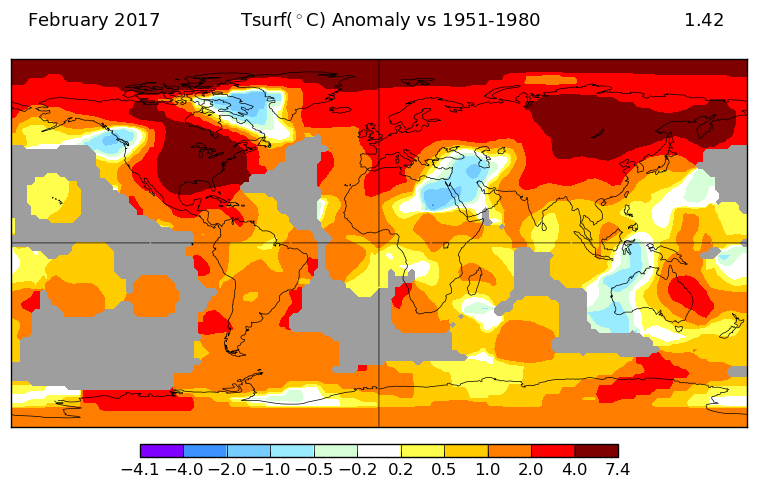
\includegraphics[width=0.92\textwidth]{Images/sampleImage.png}
\end{center}
\source{Source Here}
\end{frame}

\begin{frame}
  \frametitle{Two Column Slide (List and Figure)}
\begin{columns}
\begin{column}{0.5\textwidth}
\begin{itemize}
  \item Point 1
  \item Point 2
\end{itemize}
\end{column}
\begin{column}{0.5\textwidth}
    \begin{center}
     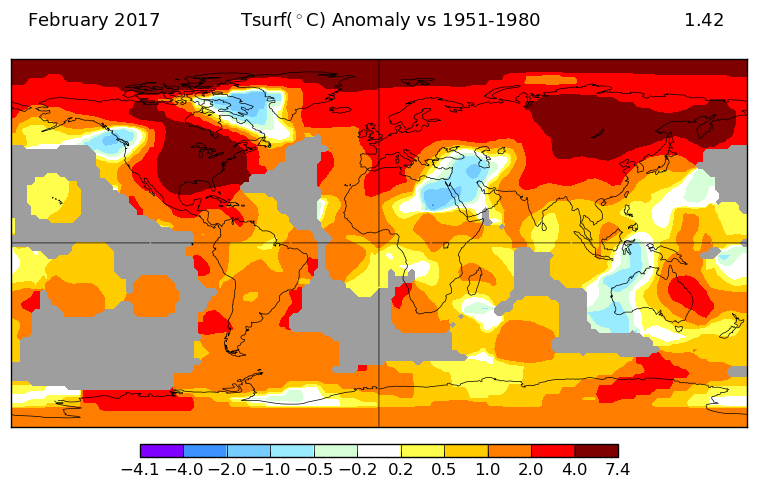
\includegraphics[width=0.95\textwidth]{Images/sampleImage.png} %merra anomaly field 
     \end{center}
\end{column}
\end{columns}
\source{Source Here}
\end{frame}


\end{document}